\section{Results}
\begin{figure*}[htb]
\centering
  \begin{subfigure}[t]{0.47\textwidth}
  \centering
  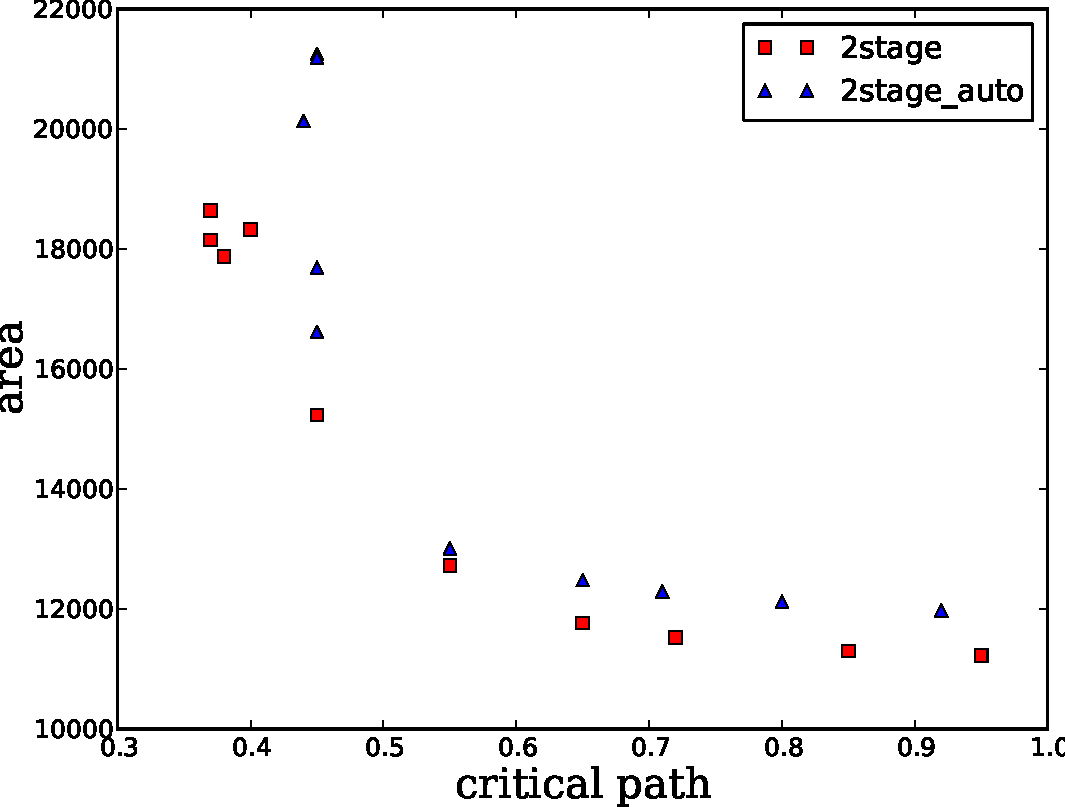
\includegraphics[width=\textwidth]{figures/2stage.pdf}
  \caption{2-stage}
  \label{fig:2stage}
  \vspace{20pt}
  \end{subfigure}
  \hfill
  \begin{subfigure}[t]{0.47\textwidth}
  \centering
  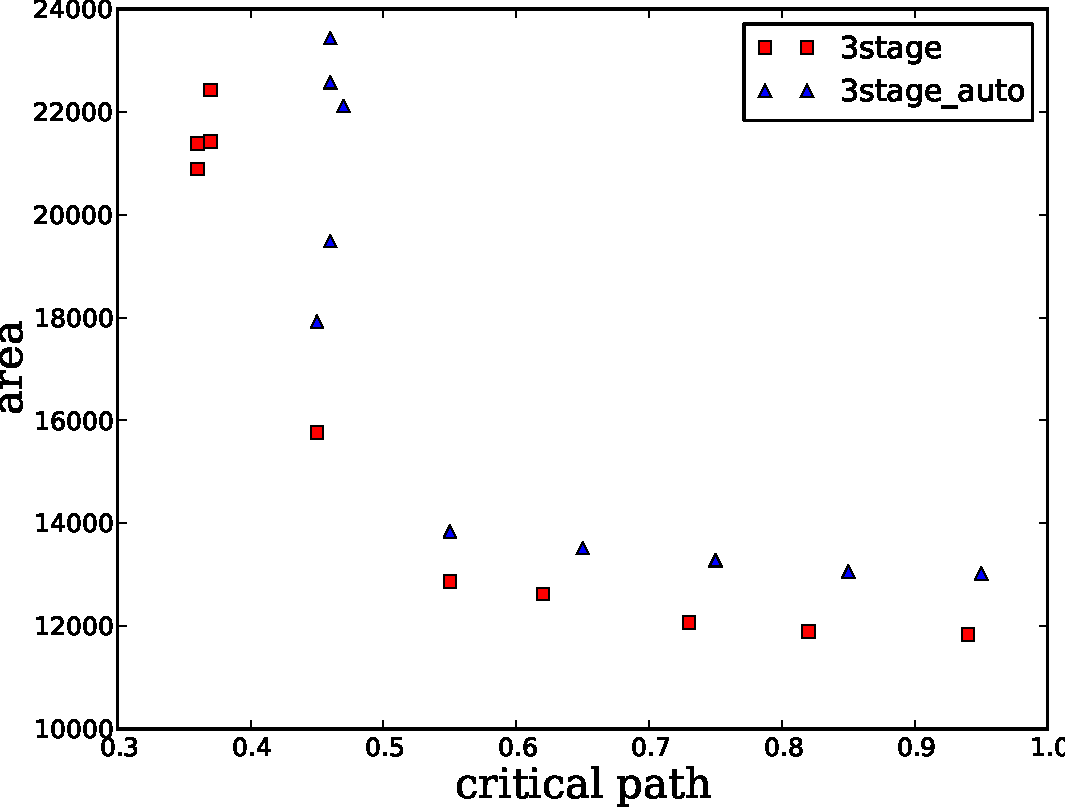
\includegraphics[width=\textwidth]{figures/3stage.pdf}
  \caption{3-stage}
  \label{fig:3stage}
  \vspace{20pt}
  \end{subfigure}
  \hfill
  \begin{subfigure}[t]{0.47\textwidth}
  \centering
  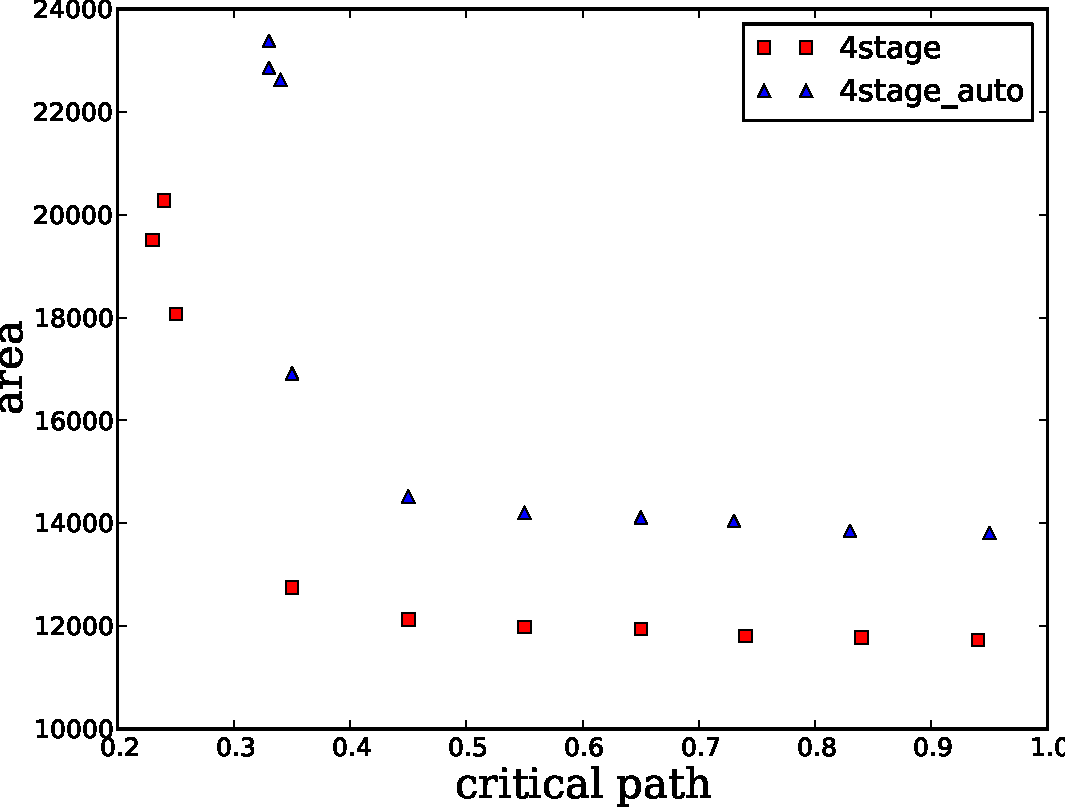
\includegraphics[width=\textwidth]{figures/4stage.pdf}
  \caption{4-stage}
  \label{fig:4stage}
  \end{subfigure}
  \hfill
  \begin{subfigure}[t]{0.47\textwidth}
  \centering
  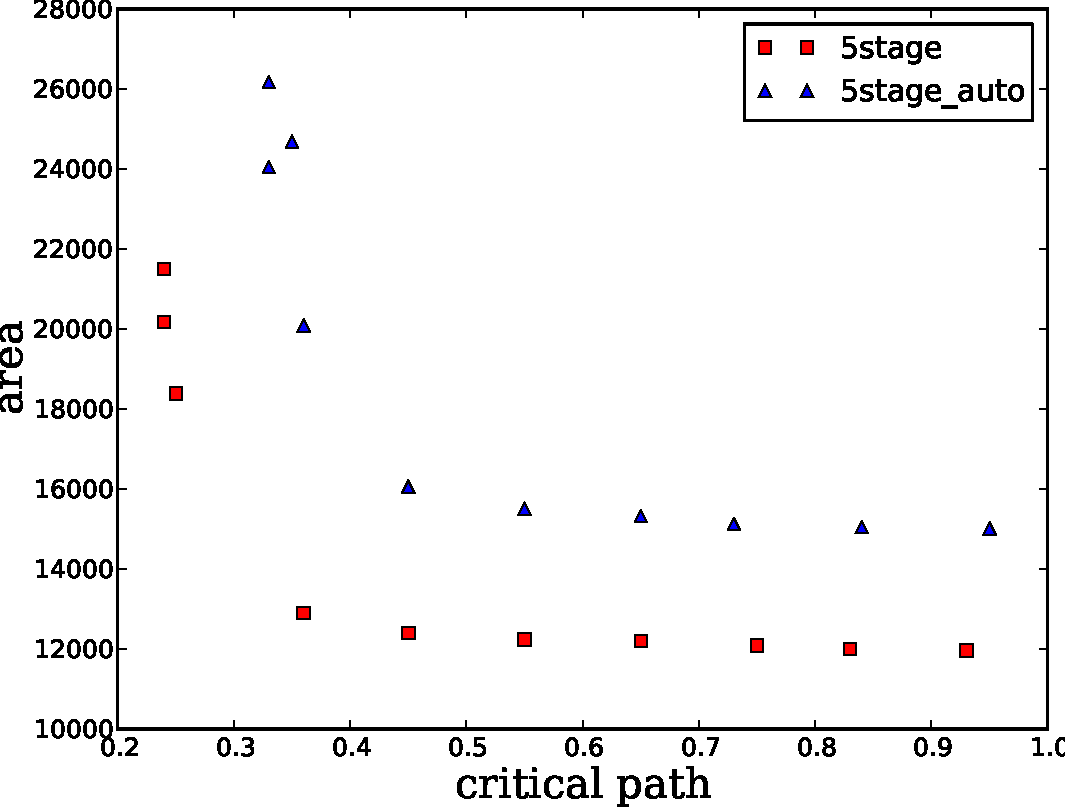
\includegraphics[width=\textwidth]{figures/5stage.pdf}
  \caption{5-stage}
  \label{fig:5stage}
  \end{subfigure}
\caption{{\bf Area vs Critical Path Comparison}. Area is measured in
  square micron. Critical path is measured in nanosecond.}
\label{fig:area-time}
\end{figure*}
\begin{figure*}[htb]
\centering
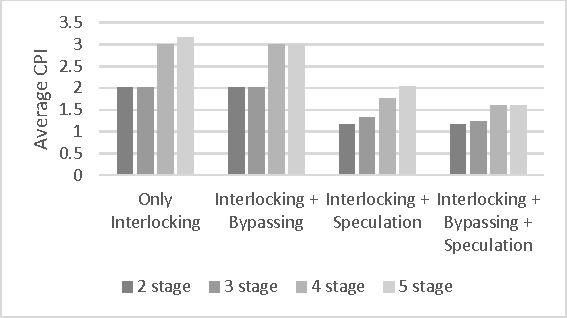
\includegraphics[trim = 25mm 175mm 60mm 0mm, clip]{figures/cpi.pdf}
\caption{{\bf CPI} averaged over the median, mixed-manufacturing, multiply, qsort, towers, and vvadd benchmarks.}
\label{fig:CPI}
\end{figure*}
To evaluate our pipeline synthesis tool, we write a 2-stage, 3-stage,
4-stage, and 5-stage pipeline specification for a single cycle CPU
datapath. We present CPI results to show that our synthesis tool is
effective in improving performance. We also push our auto-generated
pipeline through Design Compiler synthesis tool using TSMC's 45nm CMOS
library and compare the post-synthesis results to hand-coded 2-stage,
3-stage, 4-stage, and 5-stage pipelines.
\subsection{CPI}
As shown by Figure[xx], our synthesis tool does indeed improve performance by utilizing speculation and bypassing as expected. The 2-stage and 3-stage CPUs have their branches resolved in the 2nd pipeline stage and the 4-stage and 5-stage CPUS have their branches resolved in the 3rd pipeline stage. Speculation is is performed on the PC register and bypassing is performed on both read ports of the register file. There is little performance improvement from turning on bypassing without turning on speculation because most of the RAW hazards on the register file are covered up by interlocks on the PC register.
\subsection{Sodor}
Sodor is a set of simple processors written in Chisel. We use Sodor's
1-stage processor for the datapath specification. In order to work
with our tool, we modify the 1stage to use {\tt TransacationalMem}
instead of {\tt Mem} and wrapped the instruction and data cache with
our variable latency interface. Sodor also provides 2 and 5-stage
in-order processor that we use to compare against our auto-generated 2
and 5-stage processor. We had to write a 3-stage and 4-stage processor
ourselves. The hand-coded 2-stage has speculation on the PC
register. The 3, 4, and 5-stage processors make use of speculation on
the PC register and bypassing to forward results from the ALU and the
data cache.

\subsection{Comparison}
In order to see how our auto-generated pipeline holds up against a
hand-written pipeline, we push the pipelines through
synthesis. Figure~\ref{fig:area-time} compares post-synthesis results
between auto-generated pipelines and their hand-written
counterparts. We push only the CPU portion (datapath and control path,
no caches) of the processor through synthesis to better highlight the
overhead of our pipeline synthesis tool. Figure~\ref{fig:2stage} and
Figure~\ref{fig:3stage} shows that for shorter pipelines our synthesis
tool introduces little overhead. This is due to the fact that there is
very little freedom for placing pipeline registers and there are not
that many hazards to resolve. Our tool performs much worse for larger
pipelines (Figure~\ref{fig:4stage} and Figure~\ref{fig:5stage}) since
there is more freedom for register placement (which could cause our
tool to place more registers than needed) and because there are more
hazards to resolve. In particular, the 4 and 5-stage pipelines have
more bypass locations. Our tool generates an entire set of muxes for
each of these write paths instead of coalescing these write paths and
using only one mux as in the hand-coded versions.
